\chapter{Appendix E: Supporting SADb Records}\label{app:sadb_records}
\graphicspath{{figs/50-database/}}

This appendix records the curation snapshot and pathway examples supporting Chapter~\ref{ch:database}. Counts refer to the stated audited or retained set; they are not estimates of the size of the neuroscience literature.

\section{Record Sets and Coverage}

The application contains 1,393 records from the five-table base: 943 Papers, 247 Models, 157 Review Papers, 42 Feedback pathways, and 4 Recorders. Of these, 436 are archived: 382 papers and 54 non-paper records. The retained working base contains 957 records: 561 Papers, 244 Models, 109 Review Papers, 39 Feedback pathways, and 4 Recorders. The application table includes all record types, while its pivot and citation views use the paper set.

Among the 561 retained papers, 523 carry curation notes, 426 preparation tags, 240 notes assessing animal-study potential, 118 links to named feedback pathways, 86 an afferent classification, and 258 robot/simulation translation notes. There are 550 DOIs; 38 records remain without grounding text. These fields overlap and should not be summed as disjoint categories.

The citation graph was constructed over the 943-paper audit: 730 papers were connected by 11,130 directed in-corpus citation pairs, and the Louvain partition produced 18 named groups. Citation proximity supplies a navigation aid, not evidence that two papers establish the same mechanism. The citation-neighborhood view is shown in Chapter~\ref{ch:database} (Figure~\ref{fig:sadb_clusters}); Figure~\ref{fig:sadb_explorer} provides the complementary paper-table view.

\begin{figure}[htbp]
\centering
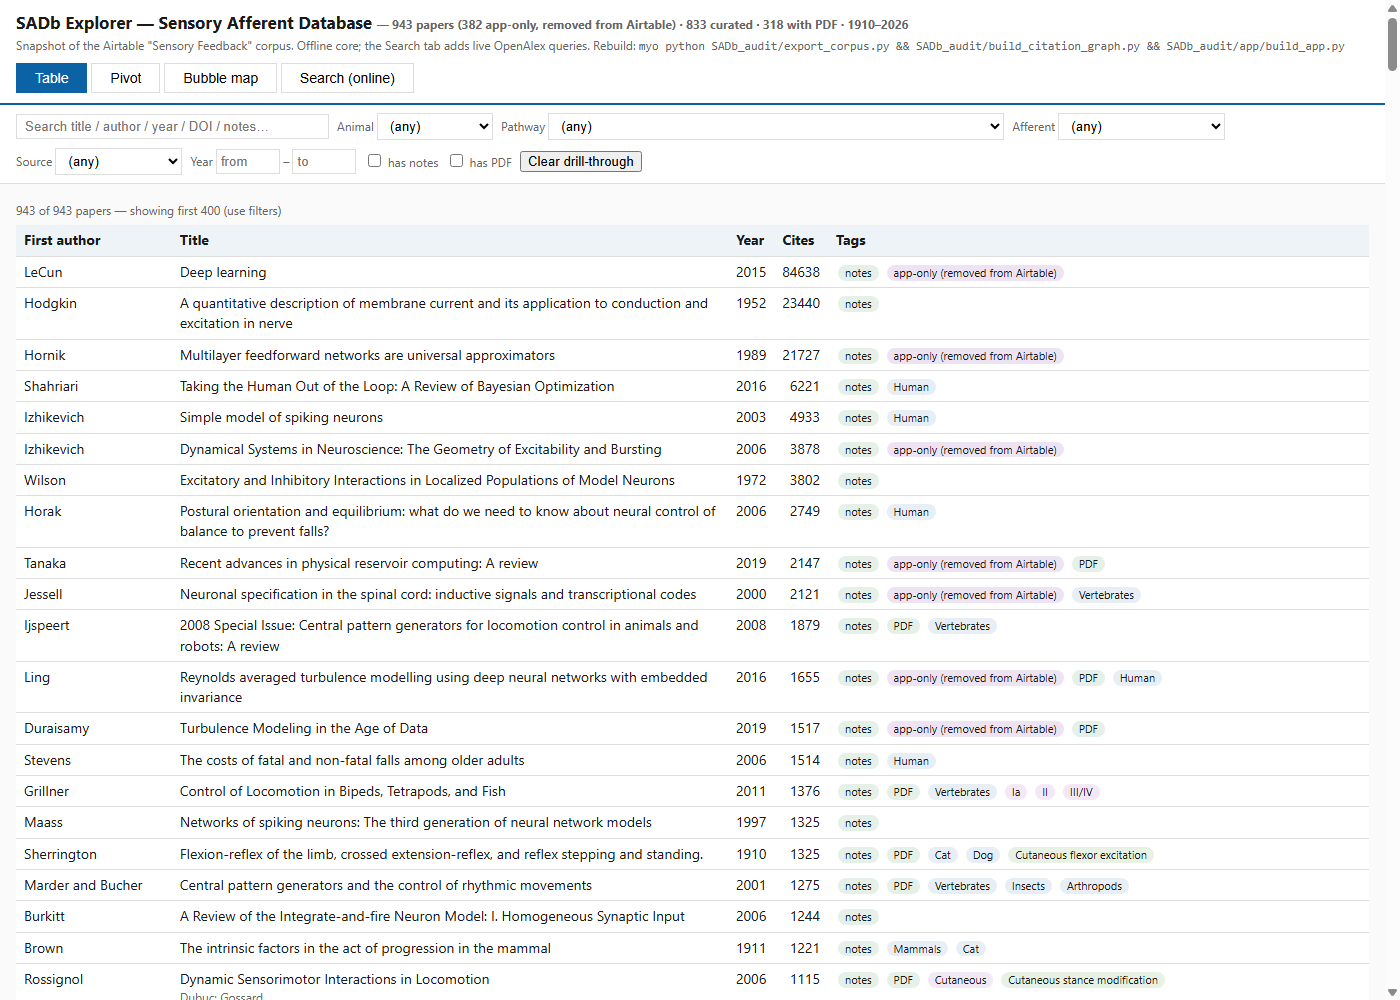
\includegraphics[width=\textwidth]{sadb_explorer.png}
\caption[The SADb Explorer]{SADb Explorer paper-table view. Searches and filters expose bibliographic information, curation notes, preparation tags, and afferent or pathway links. The embedded corpus is available offline.}
\label{fig:sadb_explorer}
\end{figure}

\section{Afferent Classes and Linked Pathways}

The tables reproduce the curated signal summaries and representative linked pathways. Their record names are database labels; pathway action depends on the experimental preparation and locomotor state described in the cited sources. Translating these records into a controller requires an explicit encoding and verification step.

\begin{table}[htbp]
\caption{Afferent classes represented in the Sensory Afferent Database, the signal each class carries, and the pathway roles the corpus records for it. Anchor references are corpus papers linked to the corresponding records; the signal summary for the Ia, II, and Ib rows follows the ensemble afferent recordings of \citet{prochazka_ensemble_1998}.}
\label{tab:sadb_afferents}
\small
\begin{tabularx}{\textwidth}{@{}>{\raggedright\arraybackslash}p{0.14\textwidth}>{\raggedright\arraybackslash}p{0.16\textwidth}>{\raggedright\arraybackslash}p{0.16\textwidth}>{\raggedright\arraybackslash}X@{}}
\toprule
\textbf{Class} & \textbf{Receptor} & \textbf{Signal carried} & \textbf{Recorded pathway roles (anchors)} \\
\midrule
Ia & muscle spindle primary & muscle length and velocity & homonymous stretch excitation \citep{eccles_integrative_1958}; reciprocal inhibition of the antagonist pool \citep{jankowska_effect_1967} \\
II & muscle spindle secondary & static muscle length & midlumbar disynaptic relay onto motor nuclei \citep{edgley_interneuronal_1987}; stance-phase support of extensor activity \citep{mazzaro_afferent_2006} \\
Ib & Golgi tendon organ & whole-muscle force & autogenic inhibition at rest, stance-phase reversal to excitation, and the load gate on swing onset \citep{dietz_significance_2000, dominguez_candidate_2020} \\
III/IV & free nerve endings & metabolic and nociceptive signals, converging with cutaneous and group II--III afferents as flexor-reflex afferents & phase-dependent resetting of the locomotor rhythm \citep{schomburg_flexor_1998} \\
Cutaneous & skin and foot-pad receptors & contact and perturbation events & flexor excitation and phase-modulated stance correction \citep{sherrington_flexion_1910, forssberg_stumbling_1979} \\
\bottomrule
\end{tabularx}
\end{table}

\begin{sidewaystable}[p]
\caption{Principal feedback-pathway records of the database's Feedback table, named by the fixed grammar of afferent, action, and phase. Linked papers are counted over the full audited corpus of 943 papers; for every pathway listed, the count is unchanged under the retained corpus of 561. Demonstrating references are the corpus papers linked to each record, as curated in the database.}
\label{tab:sadb_pathways}
\fontsize{10pt}{12pt}\selectfont
\begin{tabularx}{\textheight}{@{}llXrp{0.26\textheight}@{}}
\toprule
\textbf{Pathway record} & \textbf{Class} & \textbf{Recorded action in the step cycle} & \textbf{Linked papers} & \textbf{Demonstrating references} \\
\midrule
Ia monosynaptic excitation & Ia & stretch excitation of the homonymous motor pool, with the pathway gain modulated over the step cycle & 7 & \citep{eccles_integrative_1958, capaday_amplitude_1986} \\
Ia reciprocal inhibition & Ia & inhibition of the antagonist motor pool through the Ia inhibitory interneurons, rhythmically active in fictive locomotion & 6 & \citep{jankowska_effect_1967, pratt_ia_1987} \\
Ib disynaptic inhibition & Ib & autogenic non-reciprocal group I inhibition of the loaded muscle's own pool, reduced during stance & 5 & \citep{jankowska_common_1981, stephens_short_1996} \\
Ib disynaptic excitation & Ib & the locomotor reversal: group I input excites synergist extensor pools during the extensor phase, replacing the resting inhibition & 6 & \citep{mccrea_disynaptic_1995, pearson_enhancement_1998} \\
Ib stance to swing & Ib & the load gate: Ib input from ankle extensors prolongs stance, so swing is not initiated while the leg is loaded & 17 & \citep{dietz_significance_2000, dominguez_candidate_2020} \\
Ia or II stance to swing & Ia, II & flexor-length gate on stance termination: lengthening of flexor muscles in late stance ends extension and resets the cycle & 10 & \citep{hiebert_contribution_1996, akay_degradation_2014} \\
type II excitatory & II & stance-phase support of ankle-extensor activity through the midlumbar group II relay & 5 & \citep{edgley_interneuronal_1987, mazzaro_afferent_2006} \\
Cutaneous flexor excitation & Cutaneous & flexion withdrawal and the stumbling corrective reaction, phase-modulated over the cycle & 16 & \citep{sherrington_flexion_1910, forssberg_stumbling_1979} \\
\bottomrule
\end{tabularx}
\end{sidewaystable}
